\section{Experiments}
\begin{figure*}[t]
\centering
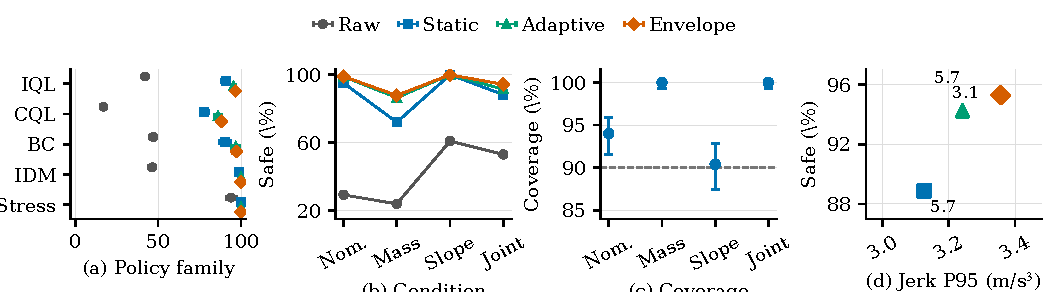
\includegraphics[width=\textwidth]{figures/fig2_evidence.pdf}
\caption{Compact evidence from ACC \emph{partial rollouts}. (a) Safety by
fixed policy family; intervals jointly resample shared reset trials.
(b) Safety across physical conditions. (c) Fresh one-step residual coverage
with exact 95\% binomial intervals; dashed line is $1-\alpha=0.9$.
(d) Safety versus comfort; point labels are mean warmed filter P95 latency
in ms. Projection rates are
6.51\%, 6.63\%, and 6.77\% for static, adaptive, and envelope filters.}
\label{fig:evidence}
\end{figure*}
\subsection{Policies, conditions, and evaluation protocol}
We evaluate four mixed-data IQL checkpoints, three mixed-data CQL checkpoints,
three independently bootstrapped linear behavior-cloning (BC) policies, an
intelligent driver model (IDM) expert, and a suboptimal-data CQL policy.
These 12 frozen policies cover
different learning objectives, training seeds, and data quality. Our real
ACC simulations are classified as \emph{partial rollout}: four conditions,
two lead-vehicle scenarios (braking and stop--go), 25 reset trials per
policy--condition--scenario cell, and a 500-step horizon. The four conditions
are $(m,\phi)=(1500,0),(1800,0),(1500,3),(1800,2)$ in kg and degrees.
All methods share initial physical states, seeds, and inference settings.
There are 2,400 paired policy--trial units and 200 distinct reset units across
the fixed policy suite.

The reduced model uses drag coefficient 0.24 and rolling coefficient 0.010,
compared with simulator values 0.30 and 0.012. The calibration model fixes
mass at 1500 kg and force gain at 0.7, using the observed grade; true force
gain is 1.0. The filter receives physical state, and the policy receives the
original normalized observation. The eight hypotheses combine
masses $\{1500,1800\}$, grades $\{0,3\}$, and force gains
$\{0.7,1.0\}$. Static and adaptive RACF use $q_\alpha=0.09188$,
obtained from the first 500 nominal calibration transitions with
$\alpha=0.1$ and $k=451$; the envelope filter uses $B=0.45$.
All three use $\eta=1$. Sequential quadratic programming solves each
projection. All data, models, and finite hypotheses are pre-generated local
assets; no external dataset enters these results. The openACC commercial
car-following database \cite{makridis2021openacc} is a natural source of future
lead-trajectory and external-coverage tests. All 12 selected checkpoints remain
frozen during evaluation.

The primary endpoint is an episode with no post-action ACC safety violation;
collisions terminate an episode. We report intervention and fallback
fractions, speed and gap RMSE, jerk P95, and warmed latency. Following
statistical guidance for RL evaluation \cite{agarwal2021precipice},
we resample reset trials jointly across policies within each
condition--scenario stratum (4,000 bootstrap draws). These intervals describe
the fixed policy suite. Exact McNemar tests \cite{mcnemar1947} compare
raw and filtered outcomes within each policy-specific cell, with Holm
correction over 288 comparisons \cite{holm1979}; the reanalysis is post hoc.
Paired intervals preserve the same resampled units \cite{efron1993}.

\begin{table}[t]
\caption{Episode-safe counts out of 600 per operating condition.
Coll. counts collisions across all 2,400 episodes per method.}
\label{tab:safety}
\centering
\setlength{\tabcolsep}{4pt}
\begin{tabular}{lrrrrr}
\toprule
Method & Nom. & Mass & Slope & Joint & Coll. \\
\midrule
Raw & 175 & 143 & 365 & 318 & 904 \\
Static & 571 & 432 & 600 & 530 & 0 \\
Adaptive & 594 & 519 & 600 & 549 & 0 \\
Envelope & 594 & 527 & 600 & 566 & 0 \\
\bottomrule
\end{tabular}

\end{table}

\subsection{Cross-policy safety and intervention}
Table~\ref{tab:safety} shows an increase from 1,001/2,400 safe raw episodes
to 2,133 static, 2,262 adaptive, and 2,287 envelope-filtered episodes.
All filtered runs complete 500 steps with zero collisions, compared with
904 collisions for raw policies. The paired safety gains are 47.17,
52.54, and 53.58 percentage points; the corresponding reset-cluster 95\%
intervals are [45.29,49.00], [51.04,54.04], and [52.21,54.96].
Across the 288 policy-specific comparisons, 149 remain significant after
Holm correction. Figure~\ref{fig:evidence}(a) shows the underlying heterogeneity:
IQL improves from 42.0\% safe episodes to 90.8--96.8\%, whereas CQL
improves from 17.0\% to 77.8--88.2\%. The suboptimal-data CQL policy
already reaches 94.0\% raw safety. Training-data quality therefore does not
by itself determine constraint pressure; the learned behavior matters.

The gains also appear in violation duration. Mean within-episode violation
fractions fall from 17.97\% for raw policies to 0.214\%, 0.122\%, and
0.095\% for static, adaptive, and envelope filtering. In nominal braking,
raw policies average 49.37 violating steps per episode, versus 0.03 for
static and zero for the other filters. Intervention is relatively sparse:
6.51\%, 6.63\%, and 6.77\% of actions are projected. Fallback occurs
on 0.91\%, 0.95\%, and 0.97\% of steps, respectively.
The envelope has 154 fewer unsafe episodes than static RACF while increasing
the projection fraction by 0.26 percentage points. These comparisons
measure operating-point effects; a margin-matched ablation is needed to
isolate the benefit of episode-level calibration itself.

\subsection{Independent coverage and control cost}
We separately evaluate one-step scores using 500 independent cruise resets
per condition, random actions, and zero to fifty random warm-up steps.
The threshold remains fixed at the value used in the closed-loop study.
The new reset seeds are disjoint from calibration and control evaluation,
and no transition duplicates any archived calibration or test record.
Coverage is 470/500 nominal (94.0\%, exact 95\% interval
[91.55,95.92]), 500/500 mass shift ([99.26,100]),
452/500 slope shift (90.4\%, [87.47,92.84]), and 500/500 joint shift
([99.26,100]); Fig.~\ref{fig:evidence}(c) summarizes these intervals. This
probe uses newly disjoint data after an audit of the
archived calibration/test split. Physical shifts can contract the residual
distribution, explaining the high mass-shift coverage.

\begin{table}[t]
\caption{Control performance on the 1,496 paired episodes where all four
methods complete 500 steps. Speed/gap: RMSE in m/s and m; jerk: mean
episode P95 in m/s$^3$; return: accumulated reward.}
\label{tab:utility}
\centering
\setlength{\tabcolsep}{5pt}
\begin{tabular}{lrrrr}
\toprule
Method & Speed & Gap & Jerk & Return \\
\midrule
Raw & 6.25 & 38.57 & 0.71 & -4934 \\
Static & 6.28 & 38.83 & 0.96 & -4624 \\
Adaptive & 6.28 & 38.85 & 1.15 & -4626 \\
Envelope & 6.28 & 38.88 & 1.24 & -4628 \\
\bottomrule
\end{tabular}

\end{table}

Raw collisions shorten the accumulation of predominantly negative rewards.
Consequently, the all-episode returns ($-4419$ raw versus approximately
$-5080$ filtered) combine performance and survival duration.
Table~\ref{tab:utility} adds a common-horizon comparison. On these paired
survivors, filtered returns improve from $-4934$ to approximately $-4626$,
while speed RMSE changes from 6.25 to 6.28 m/s. Comfort remains the
clearest cost: jerk P95 increases from 0.71 to 0.96--1.24 m/s$^3$.
This subset is a descriptive control-cost diagnostic; the full sample
remains the basis for safety reporting.



\subsection{Runtime and baseline diagnostics}
Evaluation uses four RTX 4090 GPUs for neural-policy inference and CPU
optimization for the filters. Figure~\ref{fig:evidence}(d) connects warmed
P95 latency to safety and jerk. Static, adaptive, and envelope filter P95s
are 5.72, 3.10, and 5.67 ms; their end-to-end P95s, including policy
inference, update, and environment step, are 6.07, 3.72, and 6.02 ms.
Candidate selection reduces the optimization workload in the adaptive
variant, whose update cost averages 0.25 ms. The filter P99s rise to
21.35, 11.13, and 22.28 ms, motivating explicit tail-latency measurement
when selecting a control period.

An independently implemented 20-step linear MPC provides a diagnostic
reference. Its OSQP solver \cite{osqp2020} uses constant lead-speed prediction
and soft headway constraints. Replaying the 200 distinct reset units
reproduces every recorded safety outcome; clipped force/action mapping
error stays below $1.49\times10^{-4}$ N. All 100,000 solver calls return
solved or solved-inaccurate status. MPC has zero collisions but violates
headway in every episode, illustrating the effect of lead braking on a
controller operating near the constraint boundary. Its action difference
from the learned policy is a controller deviation, so it is excluded from
the filter-intervention comparison.
